\section{Junction trees}

Several models incorporate loops, and it is feasible to transform them into a tree structure by delineating variable groups (separators) that define message interactions.
\begin{example}
    Consider the Bayesian network depicted below:
    \begin{figure}[H]
        \centering
        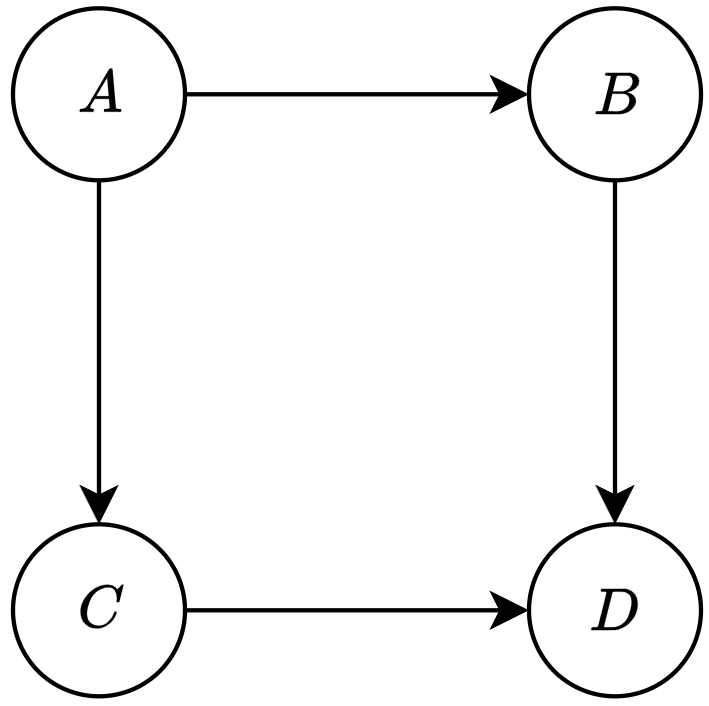
\includegraphics[width=0.25\linewidth]{images/jt.png}
    \end{figure}
    Upon applying the junction tree algorithm, the resulting structure is illustrated as follows:
    \begin{figure}[H]
        \centering
        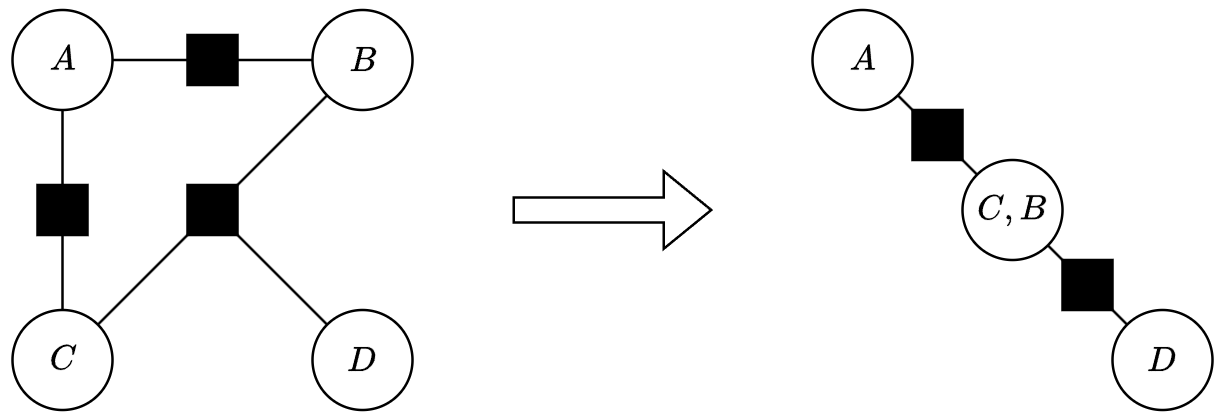
\includegraphics[width=0.5\linewidth]{images/jt1.png}
    \end{figure}
\end{example}
The process of constructing a junction tree involves the following steps:
\begin{enumerate}
    \item Moralize the graph in case it is directed.
    \item Choose a node ordering and identify cliques generated through variable elimination, thereby creating a graph triangulation.
    \item Construct a junction graph based on the eliminated cliques.
    \item Determine a suitable spanning tree.
\end{enumerate}